\documentclass[12pt,a4paper]{article}
\usepackage{graphicx}
\usepackage{xcolor}
\usepackage{array}
\usepackage{caption}
\usepackage[margin=1in]{geometry}

\definecolor{custompurple}{RGB}{200,20,200}
\colorlet{custommix}{red!60!yellow}

\title{Assignment 4 -- Lists, Colors, Figures etc.}
\author{TW Lab 2025}
\date{}

\begin{document}

\maketitle

\section{Lists}

Following are some technologies that can be used to format content:

\begin{itemize}
    \item \LaTeX
    \item HTML (+CSS)
    \item Markdown
\end{itemize}

You would most likely use \LaTeX\ in the following scenarios:

\begin{enumerate}
    \item To write research papers
    \item To embed math equations within other software (e.g. GDocs, HTML etc.)
    \item To create your CV, project reports \& presentations
\end{enumerate}

There are three main categories of electronic markup:

\begin{description}
    \item[Presentational] Used by traditional word-processing systems: binary codes embedded within document text that produce the WYSIWYG (``what you see is what you get'') effect. e.g. Microsoft Word
    \item[Procedural] Markup is embedded in text which provides instructions for programs to process the text. e.g. TEX
    \item[Descriptive] Markup is specifically used to label parts of the document for what they are, rather than how they should be processed. e.g. \LaTeX, HTML5
\end{description}

\section{Tables \& Colors}

Table 1 is placed on a separate float page using the \texttt{p} placement option.

\begin{table}[p]
\centering
\begin{tabular}{|>{\raggedright\arraybackslash}p{2.5cm}|>{\raggedright\arraybackslash}p{2cm}|>{\raggedright\arraybackslash}p{2cm}|>{\raggedright\arraybackslash}p{3.5cm}|}
\hline
Language & Requires compilation & Output & Use \\
\hline
C/C++ & Yes & Executable & To make apps \\
\hline
\LaTeX & Yes & PDF & To make documents \\
\hline
HTML/CSS/JS & No & Webpage & To make websites \\
\hline
2.5 cm & 2 cm & 2 cm & 3.5 cm \\
\hline
\end{tabular}
\caption{This table should be rendered on a special page.}
\label{tab:languages}
\end{table}

Colors can be represented using RGB values. In HTML notation, the custom RGB color can be written as \texttt{\#C814C8} or \texttt{rgb(200,20,200)}.

\[
\textcolor{custompurple}{T(n)}
=
\textcolor{custommix}{aT(n/b)+f(n)}
\]

The first custom color is defined with RGB values 200 red, 20 green, and 200 blue. The second color is made by mixing 60\% red and 40\% yellow using \texttt{\textbackslash colorlet}.

\section{Figures}

\subsection{Pictures: rotation \& cropping}

The MNIT logo is rotated to the upright position.

\begin{figure}[htbp]
\centering

\includegraphics[angle=90,width=0.32\textwidth]{mnit_logo.png}
\caption{MNIT logo}
\label{fig:mnit-logo}
\end{figure}

The building image is cropped from the top to remove the sky and is made as wide as the text.

\begin{figure}[htbp]
\centering
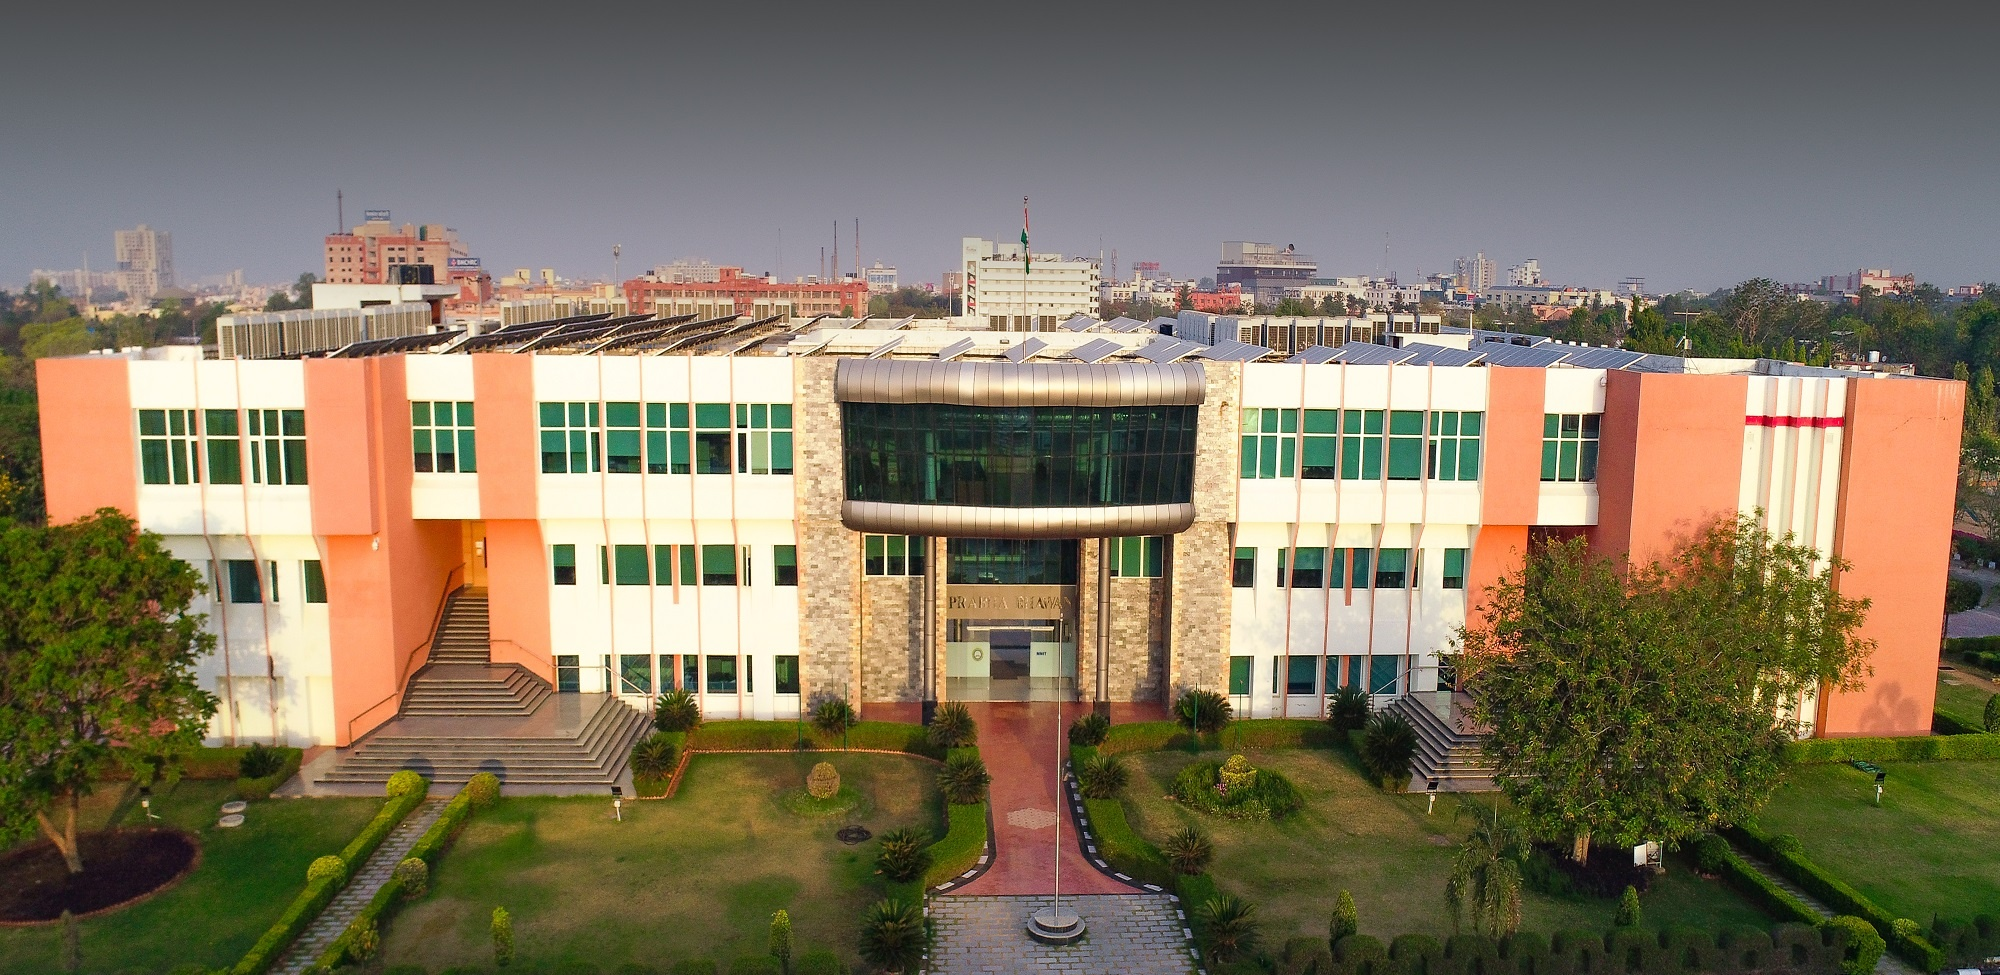
\includegraphics[width=\textwidth,trim=0 0 0 55,clip]{mnit_building.jpg}
\caption{This is a floating image and can appear anywhere.}
\label{fig:mnit-building}
\end{figure}

\subsection{Multiple images}

This subsection includes two minipages with equal width.

\begin{figure}[htbp]
\centering
\begin{minipage}[c]{0.45\textwidth}
    \centering
    
\includegraphics[width=\linewidth]{mnit_logo.png}
    \captionof{figure}{This is the first minipage}
    \label{fig:first-minipage}
\end{minipage}
\hfill
\begin{minipage}[c]{0.45\textwidth}
    \centering
    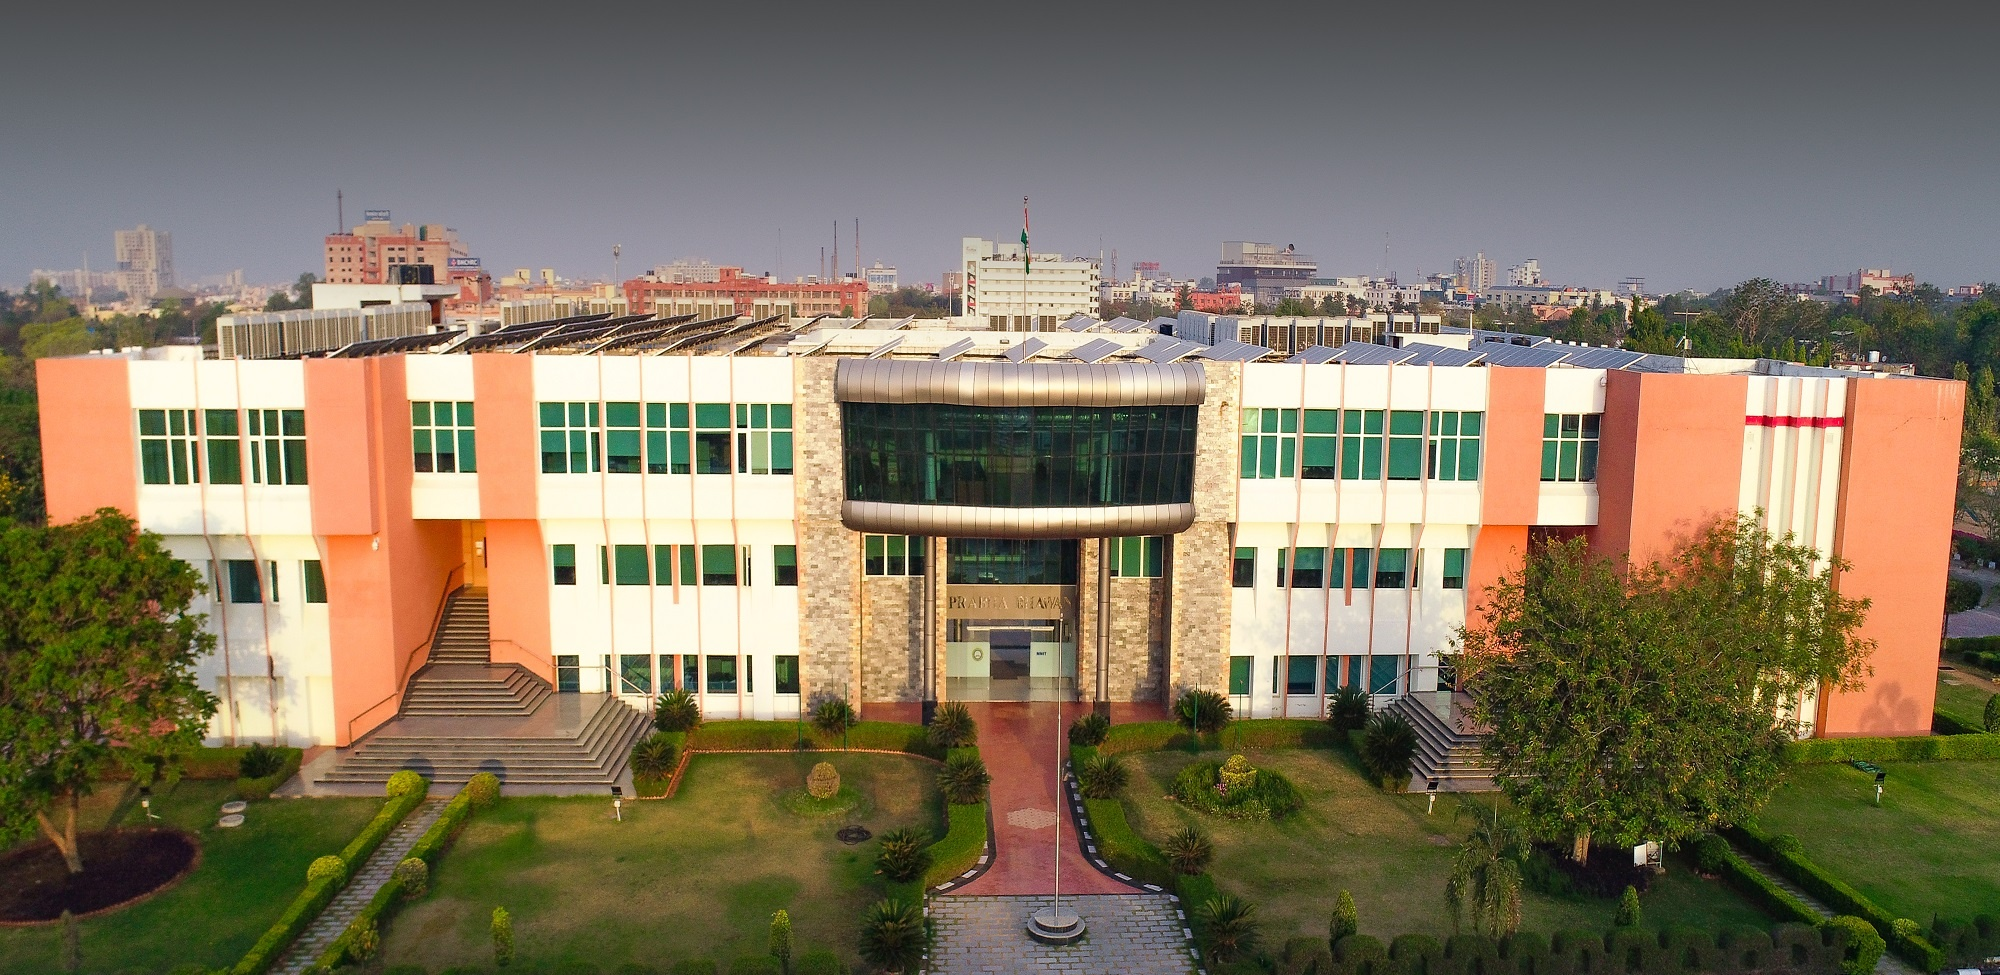
\includegraphics[width=\linewidth,trim=0 0 0 55,clip]{mnit_building.jpg}
    \captionof{figure}{This is the second minipage}
    \label{fig:second-minipage}
\end{minipage}
\end{figure}

\end{document}
